\documentclass[tikz,border=10pt]{standalone}
\usepackage{amsmath}
\usepackage{tikz}
\usetikzlibrary{shapes, arrows.meta, positioning, fit, backgrounds, calc}

\begin{document}

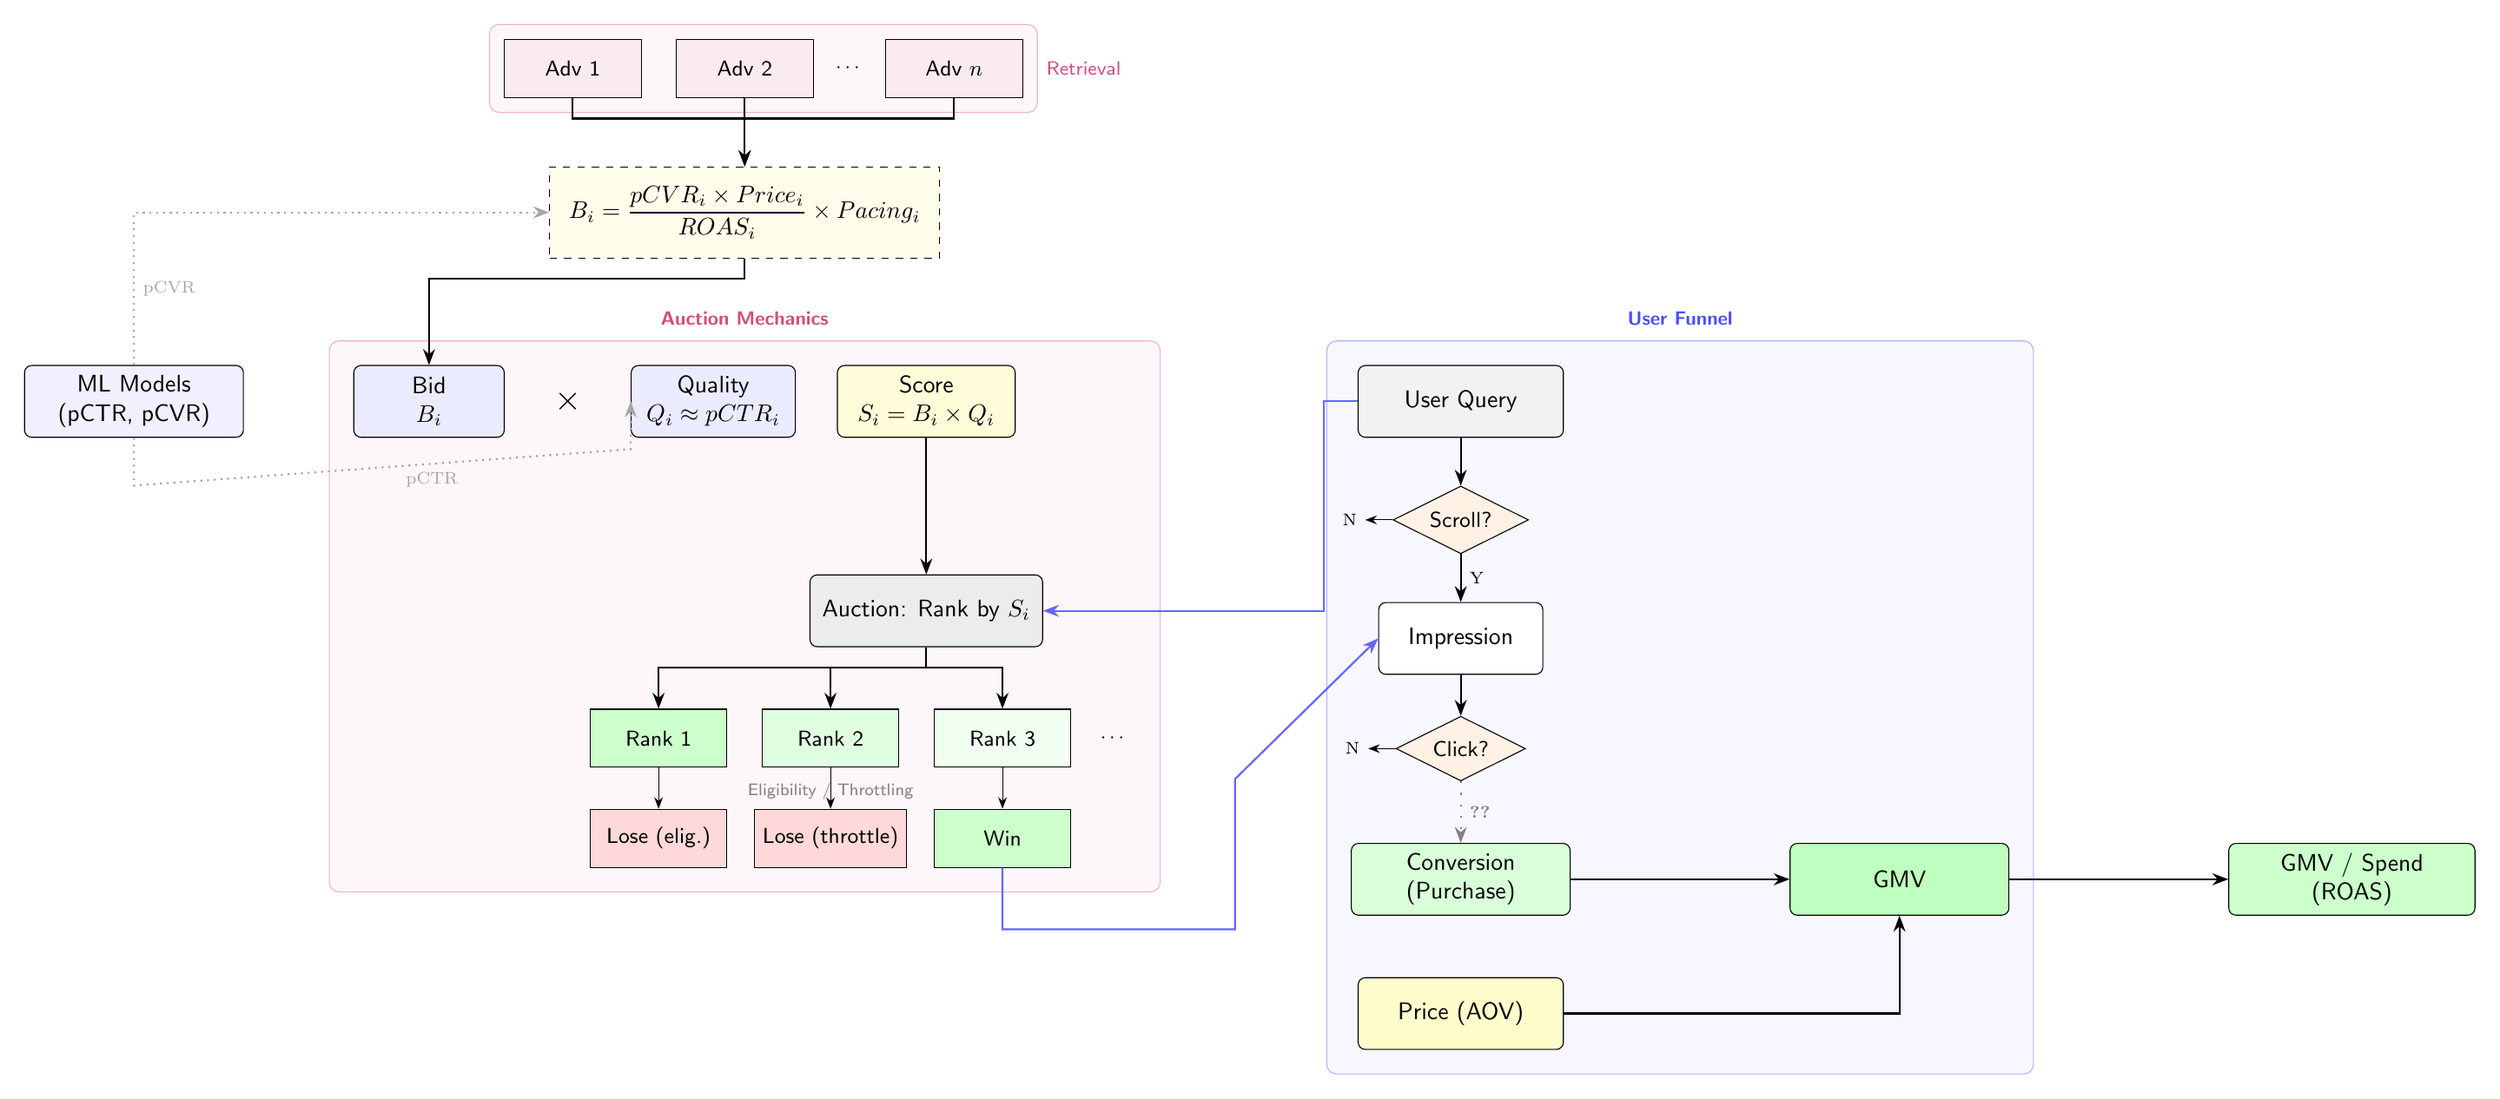
\begin{tikzpicture}[
    >=Stealth,
    node distance=1.0cm,
    box/.style={rectangle, draw, rounded corners=3pt, minimum height=1.05cm, minimum width=2.9cm, align=center, font=\sffamily\normalsize, fill=white},
    formula/.style={rectangle, draw, dashed, fill=yellow!8, align=center, font=\sffamily\normalsize, inner sep=8pt},
    smallbox/.style={rectangle, draw, minimum height=0.85cm, minimum width=2.0cm, align=center, font=\sffamily\small, fill=white},
    decision/.style={diamond, draw, fill=orange!10, aspect=2, font=\sffamily\small, inner sep=3pt},
    faint/.style={gray, font=\sffamily\scriptsize}
]

    % (Advertisers + Autobidding moved near top after labels)

    % === ROW 3: SCORING (ML later positioned left of Bid) ===
    \node (bid) [box, fill=blue!8, minimum width=2.2cm] {Bid\\$B_i$};
    \node (times) [right=0.6cm of bid, font=\Large] {$\times$};
    \node (quality) [box, right=0.6cm of times, fill=blue!8, minimum width=2.4cm] {Quality\\$Q_i \approx pCTR_i$};
    \node (score) [box, right=0.6cm of quality, fill=yellow!15, minimum width=2.6cm] {Score\\$S_i = B_i \times Q_i$};

    % === ROW 4: AUCTION (pushed further lower) ===
    \node (auction) [box, below=2.0cm of score, fill=gray!15, minimum width=3.4cm] {Auction: Rank by $S_i$};

    % === ROW 5: RANKED SLOTS ===
    \node (slot1) [smallbox, below left=0.9cm and 1.2cm of auction, fill=green!20] {Rank 1};
    \node (slot2) [smallbox, right=0.5cm of slot1, fill=green!12] {Rank 2};
    \node (slot3) [smallbox, right=0.5cm of slot2, fill=green!6] {Rank 3};
    \node (slotdots) [right=0.3cm of slot3, font=\footnotesize] {$\cdots$};

    % === ROW 6: ELIGIBILITY / THROTTLING OUTCOME (post-ranking) ===
    \node (eliglbl) [faint, below=0.1cm of slot2] {Eligibility / Throttling};
    \node (win1) [smallbox, below=0.6cm of slot1, fill=red!15] {Lose (elig.)};
    \node (win2) [smallbox, below=0.6cm of slot2, fill=red!15] {Lose (throttle)};
    \node (win3) [smallbox, below=0.6cm of slot3, fill=green!20] {Win};

    % === USER FUNNEL (right side, more horizontal spacing) ===
    \node (user) [box, right=5.0cm of score, fill=gray!10, minimum width=3.0cm] {User Query};
    \node (scroll) [decision, below=0.7cm of user] {Scroll?};
    \node (impress) [box, below=0.7cm of scroll, minimum width=2.4cm] {Impression};
    \node (click) [decision, below=0.6cm of impress] {Click?};
    % Purchase just below the user funnel; merge with AOV to GMV
    \node (conv) [box, below=0.9cm of click, fill=green!15, minimum width=3.2cm] {Conversion\\(Purchase)};
    \node (aov) [box, below=0.9cm of conv, fill=yellow!20, minimum width=3.0cm] {Price (AOV)};
    \node (gmv) [box, right=3.2cm of conv, fill=green!25, minimum width=3.2cm] {GMV};
    \node (roas) [box, right=3.2cm of gmv, fill=green!20, minimum width=3.6cm] {GMV / Spend\\(ROAS)};

    % === EDGES: AUCTION FLOW ===

    % (multiplication indicated by symbol; no direct arrow needed from Bid to Score)
    \draw[->, thick] (score.south) -- (auction.north);

    \draw[->, thick] (auction.south) -- ++(0,-0.3) -| (slot1.north);
    \draw[->, thick] (auction.south) -- ++(0,-0.3) -| (slot2.north);
    \draw[->, thick] (auction.south) -- ++(0,-0.3) -| (slot3.north);

    % Post-ranking outcomes
    \draw[->] (slot1.south) -- (win1.north);
    \draw[->] (slot2.south) -- (win2.north);
    \draw[->] (slot3.south) -- (win3.north);

    % === EDGES: USER FUNNEL ===
    \draw[->, thick] (user) -- (scroll);
    \draw[->, thick] (scroll) -- node[right, font=\scriptsize] {Y} (impress);
    \draw[->] (scroll.west) -- ++(-0.4,0) node[left, font=\scriptsize] {N};
    \draw[->, thick] (impress) -- (click);
    \draw[->] (click.west) -- ++(-0.4,0) node[left, font=\scriptsize] {N};
    % Direct but uncertain link: dotted arrow Click -> Conversion with "??"
    \draw[loosely dotted, ->, thick, gray]
        (click.south) -- node[midway, right, font=\scriptsize\bfseries, gray] {??} (conv.north);
    % Merge to GMV (equal contributions from Conversion and Price)
    \draw[->, thick] (conv.east) -- (gmv.west);
    \draw[->, thick] (aov.east) -| (gmv.south);
    % Derive ROAS = GMV / Spend
    \draw[->, thick] (gmv.east) -- (roas.west);

    % === CROSS CONNECTION: delivery path from Rank 3 Win to Impression ===
    \draw[->, thick, blue!60] (win3.south) -- ++(0,-0.9) -- ++(3.4,0) -- ++(0,2.2) -- (impress.west);
    % no path from blank (win3)
    \draw[->, thick, blue!60] (user.west) -- ++(-0.5,0) |- (auction.east);

    % === FEEDBACK === (removed per request)

    % === LABELS ===
    \begin{scope}[on background layer]
        \node[fit=(bid)(quality)(score)(auction)(slot1)(slotdots)(win2),
              draw=purple!30, fill=purple!3, rounded corners, inner sep=10pt] (abox) {};
        \node[fit=(user)(impress)(click)(conv)(gmv)(aov)(scroll),
              draw=blue!30, fill=blue!3, rounded corners, inner sep=10pt] (ubox) {};
    \end{scope}

    \node[above=0.1cm of abox.north, font=\sffamily\bfseries\footnotesize, purple!70] {Auction Mechanics};
    \node[above=0.1cm of ubox.north, font=\sffamily\bfseries\footnotesize, blue!70] {User Funnel};

    % Place ML Models left of Bid
    \node (ml) [box, left=1.6cm of bid, fill=blue!6, minimum width=3.2cm] {ML Models\\(pCTR, pCVR)};

    % === TOP ROW: Advertisers and Autobidding just above Auction Mechanics title ===
    \node (autobid) [formula, above=1.2cm of abox.north] {$B_i = \dfrac{pCVR_i \times Price_i}{ROAS_i} \times Pacing_i$};
    \node (adv2) [smallbox, above=1.0cm of autobid, fill=purple!8] {Adv 2};
    \node (adv1) [smallbox, left=0.5cm of adv2, fill=purple!8] {Adv 1};
    \node (advdots) [right=0.2cm of adv2, font=\footnotesize] {$\cdots$};
    \node (advn) [smallbox, right=0.2cm of advdots, fill=purple!8] {Adv $n$};

    % Retrieval bounding box around advertisers with right-side label
    \begin{scope}[on background layer]
        \node[fit=(adv1)(adv2)(advdots)(advn),
              draw=purple!30, fill=purple!3, rounded corners, inner sep=6pt,
              label={[font=\sffamily\footnotesize, purple!70]right:Retrieval}]
              (retrievalbox) {};
    \end{scope}

    % Edges: Advertisers -> Autobid, Autobid -> Bid
    \draw[->, thick] (adv1.south) -- ++(0,-0.3) -| (autobid.north);
    \draw[->, thick] (adv2.south) -- (autobid.north);
    \draw[->, thick] (advn.south) -- ++(0,-0.3) -| (autobid.north);
    \draw[->, thick] (autobid.south) -- ++(0,-0.3) -| (bid.north);

    % ML dotted outputs (route pCTR below Bid to Quality)
    \draw[->, dotted, gray!70, line width=0.8pt]
        (ml.south) -- ++(0,-0.7) -- node[pos=0.6, below, font=\scriptsize] {pCTR}
        ([yshift=-0.7cm]quality.west) -- (quality.west);
    \draw[->, dotted, gray!70, line width=0.8pt]
        (ml.north) |- node[pos=0.25, right, font=\scriptsize] {pCVR} (autobid.west);

\end{tikzpicture}

\end{document}
